\subsection{Design of system}
\label{sec: system}

\subsubsection{Problem Setting}
\label{sec: problem_settings}

Online Portfolio Selection is the process that one distributes his/her wealth into $m$ different financial market assets sequentially in a period of time $t$, aiming to achieve certain goals such as maximum return. The movements of an asset price usually includes open, high, low, close, volume (OHLCV) and closing price is mostly used in OLPS~\cite{li2014online}. In this work, price movement at time $t$ is defined in \emph{price relative vector}, $\vec X_{t}$. For example, the $i\mathrm{th}$ element of $\vec{X}_t$, $\vec{X}_{i,t}$ is the closing price of the $i\mathrm{th}$ asset in the $t$th period. If the market is continuous, $\vec{X}_t$ is also the opening prices at Period $t+1$. Mathematically, the \emph{price relative vector} is the ratio of $t$th closing price to previous $(t-1)$th closing price:
\begin{equation}
	\vec{x}_{t} := \vec{x}_{t} \oslash \vec{x}_{t-1} =
\left(\frac{ x_{1, t}}{x_{1, t-1}}, \frac{x_{2, t}}{x_{2, t-1}}, ..., \frac{x_{m, t}}{x_{m, t-1}} \right)^\intercal.
\label{eq:x}
\end{equation}

The portfolio value $P$ at the end of Period $t$ without considering transaction cost is thus calculated as the product of market sequence $X$ and portfolio weight vector $\vec w$,
\begin{equation} \label{eq:portfolio_value_t_no_cost}
    P_{t} = \prod_{t-1}^{i=0} \vec{x}_{i+1} \bcdot \vec{w}_{i},
\end{equation}

The sum of $\vec{w}_t$ is always 1 when leverage and short are not considered.
$\forall t, \sum\limits_i  w_{t,i} =1$. Then we can calculate the \emph{rate of return}(RoR) as, 
\begin{equation} \label{eq:rho_t_no_cost}
	\rho_{t} := \frac{P_{t}}{P_{t-1}} = \vec{x}_{t} \bcdot \vec{w}_{t-1}
\end{equation}

The \emph{gross logarithmic rate of return} is simply apply logarithmic function to RoR, mathematically,
\begin{equation} 
    \mathrm{log}r_{t} := \ln \frac{P_{t}}{P_{t-1}} = \ln \vec{x}_{t} \bcdot \vec{w}_{t-1}.
	\label{eq:log_r_no_cost}
\end{equation}
Therefore, the final portfolio value will be
\begin{equation}\label{eq:final_P_no_cost}
	P_\mathrm{f} = P_0 \exp\left( \sum\limits_{t=1}^{t+1} r_{t} \right) = P_0 \prod_{t=1}^{t+1} \vec{x}_{t} \bcdot \vec{w}_{t-1},
\end{equation}
where $P_0$ is the initial investment amount.

By maximizing rate of return of each period, the final accumulative return is expected to be maximized as well. The general OLPS framework is as following:

\begin{algorithm}[H]
\SetAlgoLined
\SetKwInOut{Input}{Input}
\SetKwInOut{Output}{Output}
\Input{$\vec{x}_t^0$ Historic price data sequences}
\Output{$p_\mathrm{f}$ Final Portfolio Value}
{Initialize $\vec{w}_0 = (\frac{1}{m},\ldots,\frac{1}{m})$}

 \For{$t=1,2,\ldots,n$}{
  Portfolio weight vector $\vec{w}_t$ is calculated by the algorithm.\;
  Price data $x_t$ is revealed.\;
  Portfolio value vector at Period $t$ is computed as Eq~\ref{eq:portfolio_value_t_no_cost} indicates.\;
 }
 \caption{Online Portfolio Selection Framework Overview}
\end{algorithm}

There are three assumptions widely used in previous works~\cite{jiang2017deep, li2014online} and are also adopted in this work,
\begin{enumerate}
\label{num:assumptions}
    \item Transaction cost: it is assumed that no transaction cost/slippages incurred during online trading.
    \item Market liquidity: it is assumed that market liquidity is high enough, that the agents are able to buy/sell assets according to their algorithms.
    \item Market impact: it is assumed that the investments made by agents have zero influence on the price movement of the market.
\end{enumerate}

\subsubsection{Deep Reinforcement Learning Algorithm}
\label{subsub: drl}

This section presents a deep reinforcement learning algorithm to OLPS problem as Section~\ref{sec: problem_settings} describes, specifically a deep deterministic policy gradient algorithm. At the context of reinforcement learning, an agent interacts with its environment. For OLPS, the agent is the software or trading robot and the corresponding environment is certain financial market~\cite{jiang2017deep}. The agent makes an action which is buying/selling one or more assets. Mathematically,
\begin{equation}  \label{eq:action}
	\vec a_t = \vec{w_t}.
\end{equation}
where $w_t$ is the \emph{portfolio weight vector} at Period $t$. The action once made will influence the current situation. While in this work, $\vec{w}_{t-1}$ will include the influence as a part of policy making, the state therefore is represented as the pair of $X_t$ and $\vec{w}_{t-1}$,
\begin{equation} \label{eq:state}
	\vec s_t = (\bm X_t, \vec w_{t-1}),
\end{equation}
where $\vec w_0$ is predetermined by the algorithm. A policy is a mapping from state to action, $\pi:\mathcal{S}\rightarrow\mathcal{A}$. With gradient ascent, the optimal policy is made from a set of parameters $\vec{\theta}$ and the action will be $\vec a_t = \pi_{\vec \theta}(\bm s_t)$. The optimal policy will maximize the reward function from time interval $[0,t_\mathrm{f}]$, and performance metrics $J$ of $\pi_{\vec \theta}$ is the reward function from $t=0$ to $t=\mathrm{f}$:
\begin{equation}
	J(\pi_{\vec \theta}) = R\left( \vec s_1,\pi_{\vec \theta}(s_1),\cdots,
		\vec s_{t},\pi_{\vec \theta}(s_{t}),\vec s_{t+1} \right).
	\label{eq:policy_value}
\end{equation}
Then the parameters are updated by gradient descent method, towards the optimal direction,
\begin{equation}
	\vec\theta \longrightarrow \vec\theta + \lambda\nabla_{\vec\theta}J(\pi_{\vec \theta}).
	\label{eq:gradient_ascent}
\end{equation}
where $\lambda$ is the learning rate.

The reward function $R$ is the average logarithmic cumulated return for $n$ periods, expressly,
\begin{align}
	R &= \frac{1}{n} \sum_n \ln \vec x_{t} \bcdot \vec w_{t-1} \\
	  &= \frac{1}{n} \sum_n \mathrm{log}r_t
\end{align}

\subsubsection{Neural Networks and Policies}

Different neural networks are used to construct the policy $\pi_{\vec \theta}$, including Convolutional Neural Networks~\cite{lecun1998gradient}, Long-Short term Memory Networks~\cite{hochreiter1997long} and Recurrent Networks~\cite{jordan1986attractor}. Besides, several novel designs such as Identical Independent Evaluators (IIE), Ensemble of IIE (EIIE), Portfolio-Vector Memory (PVM), Online Stochastic Batch Learning (OSBL) are applied inside the network~\cite{jiang2017deep}. 

EIIE topology means the neural networks output directly to the \emph{portfolio weight vector} $\vec{w}_t$ via softmax function. PVM saves the previous portfolio weights and takes them as input for next period of training. OSBL selects the mini-batch by a geometric distribution, simply the more recent price data will be selected more frequently.


\subsubsection{Design of the Python Package}

With the basic understanding of the algorithm, this section describes some functionalities of our python package \textit{mercurius}. The example is performed on futures contract market with data available online\footnote{project url: https://github.com/dexhunter/eco301}. There are 10 assets for selection and we select several traditional algorithms to test. The input price movements is shown as Figure~\ref{fig:input_data}.

\begin{figure}
    \centering
    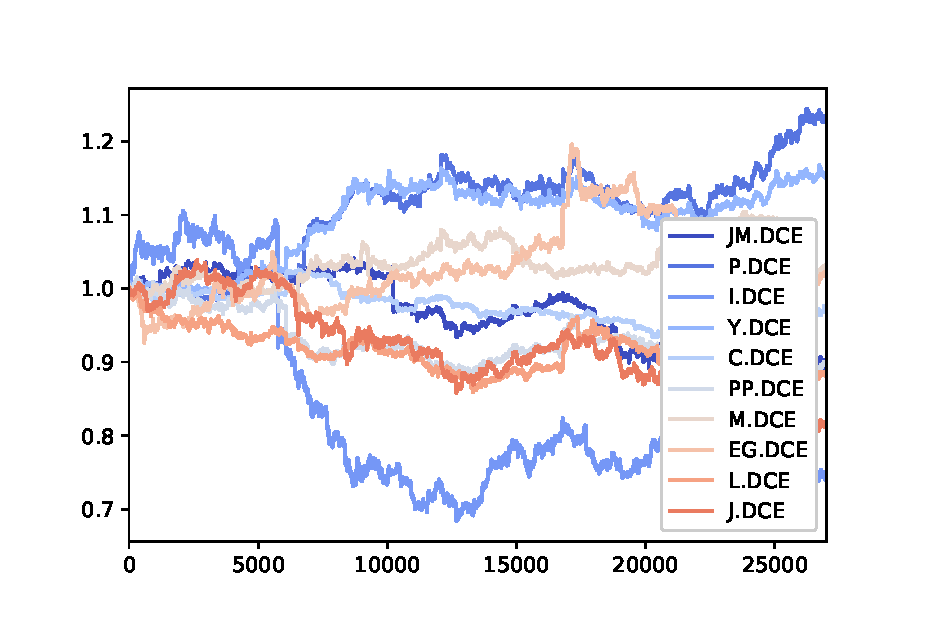
\includegraphics{img/input.eps}
    \caption{Input Sequence Data from Futures Contract Market, 10 assets are contracts for coking coal, palm oil, iron ore, soybean oil, corn, polypropylene, soybean meal, ethylene glycol, plastic and coke respectively}
    \label{fig:input_data}
\end{figure}

The performances of different algorithms is compared at Figure~\ref{fig:algo} where we select Buy-and-Hold (BAH), Constant Rebalanced Portfolio (CRP) as benchmark. Robust Median Reversion (RMR) performs the best in terms of final APV. The numeric table is demonstrated at Table~\ref{tab:my_label}. 

\begin{figure}
    \centering
    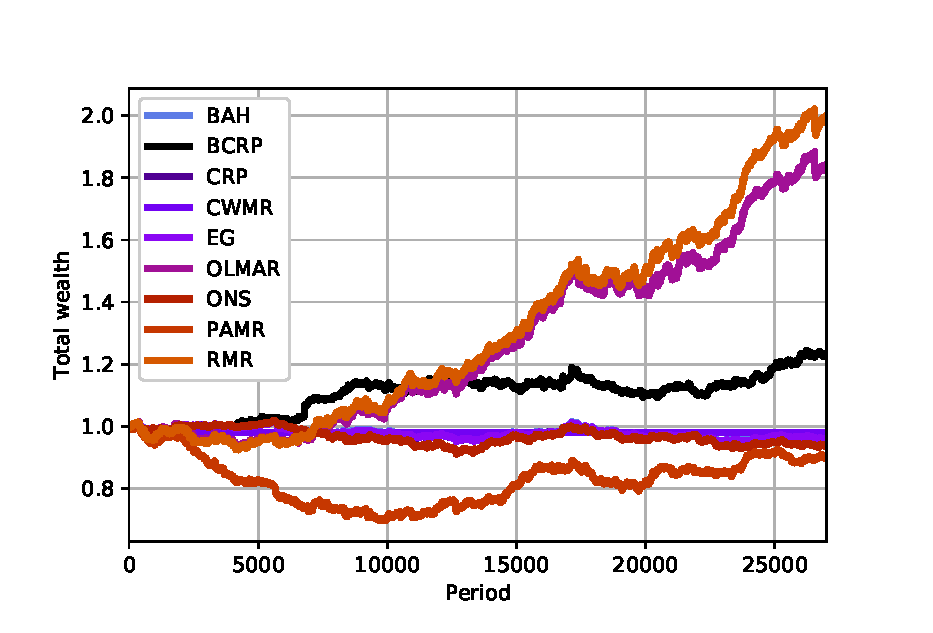
\includegraphics{img/algos.eps}
    \caption{Comparison of traditional machine learning techniques on Futures Contract Market}
    \label{fig:algo}
\end{figure}

\begin{table}[]
    \centering
\begin{tabular}{lrrrr}
\toprule
{} &   profit &    sharpe &           APV &  VaR(90\%) \\
\midrule
BAH   &  0.98876 &  -1.07573 & -9.885370e+00 &  -0.00045 \\
BCRP  &  1.03393 &   2.89564 &  7.971866e+01 &  -0.00094 \\
CRP   &  0.98824 &  -1.14052 & -1.063131e+01 &  -0.00046 \\
CWMR  &  1.42910 &   4.71027 &  2.044639e+01 &  -0.00018 \\
EG    &  0.98825 &  -1.13839 & -1.060031e+01 &  -0.00046 \\
OLMAR &  1.54763 &  38.42997 &  3.673105e+06 &  -0.00114 \\
ONS   &  0.98814 &  -1.18334 & -1.485441e+01 &  -0.00064 \\
PAMR  &  1.65176 &  44.91529 &  1.530392e+07 &  -0.00108 \\
RMR   &  1.57637 &  39.98359 &  5.552418e+06 &  -0.00113 \\
\bottomrule
\end{tabular}

    \caption{Traditional Machine Learning Techniques on Futures Contract Market}
    \label{tab:my_label}
\end{table}



\subsection{Design of evaluation}
\label{sec: evaluation}

All the algorithms mentioned at Section~\ref{subsub: background} will be backtested, in other words, historic data will be used to simulate a trading environment for algorithm to trade as if it sees the data points in real time. One caution there is to avoid look-ahead bias since the algorithm should receive the price data in a sequence. During backtesting, multiple metrics including accumulative portfolio value (APV), Sharpe ratio (SR), Maximum drawdown (MDD) are applied to measure the performance of different OLPS algorithms. To fairly compare portfolio values of different algorithms, APV is divided by the corresponding unit of the initial portfolio values:
\begin{equation}
    p_t = p_t / p_0.
\end{equation}
where $p_t$ is the accumulative portfolio value at time $t$ and $p_0$ is the initial portfolio value and will be set to $0$ after this division. APV reflects the profitability of an algorithm, however, it lacks risk information for the algorithm. Sharpe ratio and maximum drawdown, therefore, are taken into consideration for risk measurements. SR~\cite{sharpe1964, sharpe1994} considers the volatility of the portfolio values for both upwards and downwards movements, while MDD~\cite{blanchard1979MaxDD, magdon2003maximum} calculates the largest loss from a peak to a trough. Rigorously, SR is defined as the average of risk-free return by its deviation,
\begin{equation} \label{eq:sharpe}
    S = \frac{\overline{p}_t - p_f}{\sigma_p},
\end{equation}
where $\overline{p}_t$ is the expected portfolio return at time $t$, $p_f$ is the risk free rate of return (0 in this case), and $\sigma_p$ is the standard deviation of the portfolio value. For maximum drawdown, mathematically:
\begin{equation} \label{eq:mdd}
	D = \max_{\substack{\tau>t\\ t}} \frac{p_t-p_\tau}{p_t}.
\end{equation}

While in this work, more recent data from broker markets will be used. For example, forex data from October 2018 to October 2019 will be put into back-testing while training data will be from earliest available data points from broker\footnote{This work uses forex data provided by OANDA APIs}.

